\chapter{A Conceptual Model of the Carbon Cycle}
\label{chapter:conceptual_carbon_cycle}
\graphicspath{{box_ocean/figs/}}

In \cref{chapter:global_bomb}, I showed that there were conditions under which the climate was unstable,
driven by an instability in the terrestrial carbon cycle. In that chapter I found that the effects of
the biogeochemical feedback were small at the global scale. I also used a parameter $\chi_0$ to model the ocean,
which is a obvious simplification.

In this chapter then, I will construct a model of the climate-carbon system which is analytically tractable
with a dynamical ocean component but neglects the role of biochemical heating.

\section{Background}

\subsection{Climate Response to Radiative Forcing}
When certain gases, known as Greenhouse Gases, are emitted into the atmosphere they can affect global temperatures.
They do this by absorbing infrared radiation emitted by the Earth's surface and reradiating it to space at a lower temperature.
The effect of this is that less energy is radiated away to space than it did before the emission of greenhouse gases. To be in
equilibrium, the energy recieved from the Sun must equal the energy radiated to space by the Earth. As less radiation is now
emitted to space the Earth's climate responds to restore equilibrium. It does this by warming up to increase the amount it
radiates to restore equilibrium.

The amount that a greenhouse gas decreases the outgoing radiation to space by is known as its radiative forcing. If $T$ is
the global mean temperature and $N(T)$ is the net radiation recieved by the Earth (in equilibrium $N$ is zero) then for a small
radiative forcing $\Delta N$ the change in global mean temperatures is
\begin{equation}
  \label{eq:response_to_radiative_forcing}
  \Delta N = \pdv{N}{T} \Delta T.
\end{equation}
The quantity
\begin{equation}
  \label{eq:climate_sensitivity}
  \lambda = -\pdv{N}{T}
\end{equation}
known as the \emph{climate sensitivity} determines the amount of warming experienced for a given radiative forcing. This quanity is measured
in units \si{\watt\per\square\meter\per\kelvin} but it has become common to discuss $\lambda$ in terms of a given radiative forcing, $Q_{2\times}$,
the radiative forcing due to doubling the concentration of $\ce{CO2}$ in the atmosphere, giving rise to
\begin{equation}
  \label{eq:definition_of_ECS}
  \mathrm{ECS} = \frac{Q_{2\times}}{\lambda}
\end{equation}
known as \emph{Equilibrium Climate Sensitivity} which is measured in \si{\kelvin}.

Implicit in this definition is the idea that $Q_{2\times}$ is well defined. It is an empirical fact that over a range of concentrations the radiative forcing
of $\ce{CO2}$ varies with the logarithm of its concentration, and so the notion of a radiative forcing due to doubling is well defined. It is also usually assumed that
$\mathrm{ECS}$ is a constant independent of background climate state. Whilst this appears to be a good approximation, it has been challenged.

The value of $\mathrm{ECS}$ is uncertain. State of the art climate models (CMIP6) do not agree on its value, and give a range of \SIrange{1.8}{5.6}{\kelvin}, which represents an
increase in uncertainty from CMIP5. However, these estimates should be combined with other observational estimates as well as paleoclimate records. Doing this sort of
analysis leads the IPCC to conclude that the best estimate of $\mathrm{ECS}$ is \SI{3.0}{\kelvin} with a likely range of \SIrange{2.5}{4.0}{\kelvin}.

\subsection{Terrestrial Carbon Cycle Response to \ce{CO2}}
Whilst the above disussion of $\mathrm{ECS}$ treats the amount of $\ce{CO2}$ in the atmosphere as a given quantity, in reality it is also affected by the climate
system, which determines the fluxes of carbon into and out of the atmosphere through biogeochemical cycles.

On human-relevant timescales, these fluxes are controlled by terrestrial and ocean processes. The terrestrial part of the carbon cycle is controlled by the biosphere.
Carbon enters the biosphere through photosynthesis and leaves via respiration. Respiration can be subdivided into \emph{autotrophic} and \emph{heterotrophic}.
These relate to repiration done by plants (which produce their own food which hence the name \emph{auto}troph) and non-plants respectively. Heterotrophic respiration
is primarily performed by soil microbial communites which decompse the organic matter deposited into the soil from plants.

This means that the net carbon flux into the biosphere due to plants called \emph{Net Primary Productivity} (NPP) is given by the difference between photosynthesis and
autotrophic respiration. The overall carbon flux between the land and the atmosphere is therefore the difference between NPP and heterotrophic respiration. There are two key feedbacks
on NPP and heterotrophic respiration related to elevated \ce{CO2} levels that I will discuss.

Firstly, increasing $\ce{CO2}$ increases the amount of carbon availiable for plants to photosynthesise. This means that if a plant's photosynthetic activity is limit by
$\ce{CO2}$ (as opposed to light or nutrients) then increases \ce{CO2} will increase NPP. This \emph{\ce{CO2} fertilisation effect} has been detected. It acts as a negative feedback
on global warming as it tends to decrease the amount of \ce{CO2} in the atmosphere by increasing photosynthesis. This feedback is expected to decrease with increased $\ce{CO2}$ as
fewer plants become limited by avaliable carbon.

Secondly, the decomposition of organic matter is a biochemical process that depends on temperature. In particular, increasing the temperature of the decomposition reaction
will increase the rate of this reaction. Hence as $\ce{CO2}$ has a warming effect the amount of respiration will increase. This means there will be a larger flux of carbon to the
atmosphere and so this is a positive feedback. Many biological reactions are assumed to depend exponentially on temperature, increasing in rate by a factor $Q_{10}$ for every
\SI{10}{\kelvin} of warming. It is generally thought that $Q_{10} \approx 2$.

The net effect of these two feedbacks is that the terrestrial response to \ce{CO2} is uncertain as the sign of the response depends on the relative magnitude of these effects. Overall it
is thought that the heterotrophic respiration effect is larger, which leads to a net positive feedback on the climate system.

\subsection{Potential For Runaway}
Combining these two sensitivities gives the potential for a runaway effect. Consider the following situation. Suppose some carbon is transferred from the land to the atmosphere. Then the globe
will warm. As the feedback from the land is positive more carbon will be released into the atmosphere leading to further warming and more carbon released. This cycle could continue until all the
carbon from the land has been released into the atmosphere. The fact that there is carbon on land therefore tells us something about the magnitudes of the land carbon feedback and the climate sensitivity.
To make progress analysing this we must include the effect of the other store of carbon: the ocean.

\section{Ocean Model}
I will neglect temperature and chemical feedbacks on the ocean response and assume it behaves linearly to elevated \ce{CO2} levels. I will further assume that the ocean carbon carbon uptake
can be viewed as $N$ non-interacting boxes which each respond over a timescale $\tau_i$ where $i$ indexes the boxes. A fraction $f_i$ of the total carbon
flux will enter the $i$th box. I will give a post-hoc justification for this in that this model can capture the observed carbon uptake of the oceans since pre-industrial times and
will qualitatively reproduce the results of a more complex ocean model. The model I introduce here has the advantage that it can be treated analytically.

The change in carbon stored in the $i$th box, $C_i$, is given by
\begin{equation}
  \label{eq:ocean_box_i}
  \dv{C_i}{t} = f_ik \Delta C_a(t) - \frac{C_i}{\tau_i},
\end{equation}
where $k=\SI{0.2}{\per\year}$ gives the timescale of the ocean uptake and $\Delta C_a$ is the change in atmospheric carbon from its equilibrium value.

For a given $C_a(t)$ \cref{eq:ocean_box_i} can be solved in quadratures to give
\begin{equation}
  \label{eq:solution_for_box_i}
  C_i(t) = \int_0^t f_ik e^{-s/\tau_i} \Delta C_a(t - u) \dd{u},
\end{equation}
if $C_i(0) = 0$.


The overall ocean response is therefore
\begin{equation}
  \label{eq:ocean_response}
  \Delta C_o(t) = \sum_{i=1}^N \int_0^t f_ik e^{-s/\tau_i} \Delta C_a(t - s) \dd{s}.
\end{equation}
or
\begin{equation}
  \label{eq:ocean_response_in_terms_of_G}
  \Delta C_o(t) = \int_0^t G(s) \Delta C_a(t-s) \dd{s}
\end{equation}
where
\begin{equation}
  \label{eq:ocean_greens_function}
  G(t) = \sum_{i=1}^{N} f_ik e^{-t/\tau_i}
\end{equation}
is the impulse response function for the uptake of ocean carbon.

\subsection{Parameter Estimation}
\Cref{eq:ocean_response} can then be fitted to observed changes in ocean carbon\todo{give details} to estimate the
parameters $f_i$ and $\tau_i$. I will do this for a one box model, in which only $\tau_1$ needs to be estimated and
for a two box model where $\tau_1$,$\tau_2$ and $f_1$ must be estimated. The quantity $f_2$ is determined by the requirement that $f_1 + f_2 = 1$.
\begin{table}
  \centering
  \begin{tabular}{@{}lll@{}}
    \toprule
    \multicolumn{1}{c}{Parameter} & \multicolumn{2}{c}{Estimated Quantity} \\
    \cmidrule{2-3}
                                  & One Box         & Two Box              \\
    \midrule
    $\tau_1$                      & \SI{3.7}{\year} & \SI{0.5}{\year}      \\
    $\tau_2$                      &                 & \SI{124}{\year}      \\
    $f_1$                         & $1$             & $0.9$                \\
    $f_2$                         & $0$             & $0.1$                \\
    \bottomrule
  \end{tabular}
  \caption{Parameter Estimates for one and two box ocean models}
  \label{tab:one_and_two_box_parameters}
\end{table}
Taking ocean carbon sink data and atmospheric \ce{CO2} data from the global carbon budget from the year 1781 onwards (which is
when the ocean sink data is avaliable) and assuming that ocean carbon and atmospheric carbon is in equilibrium in this year I perform a
least squares fit to the one and two box models giving the parameter estimates shown in \cref{tab:one_and_two_box_parameters}.

\begin{figure}
  \centering
  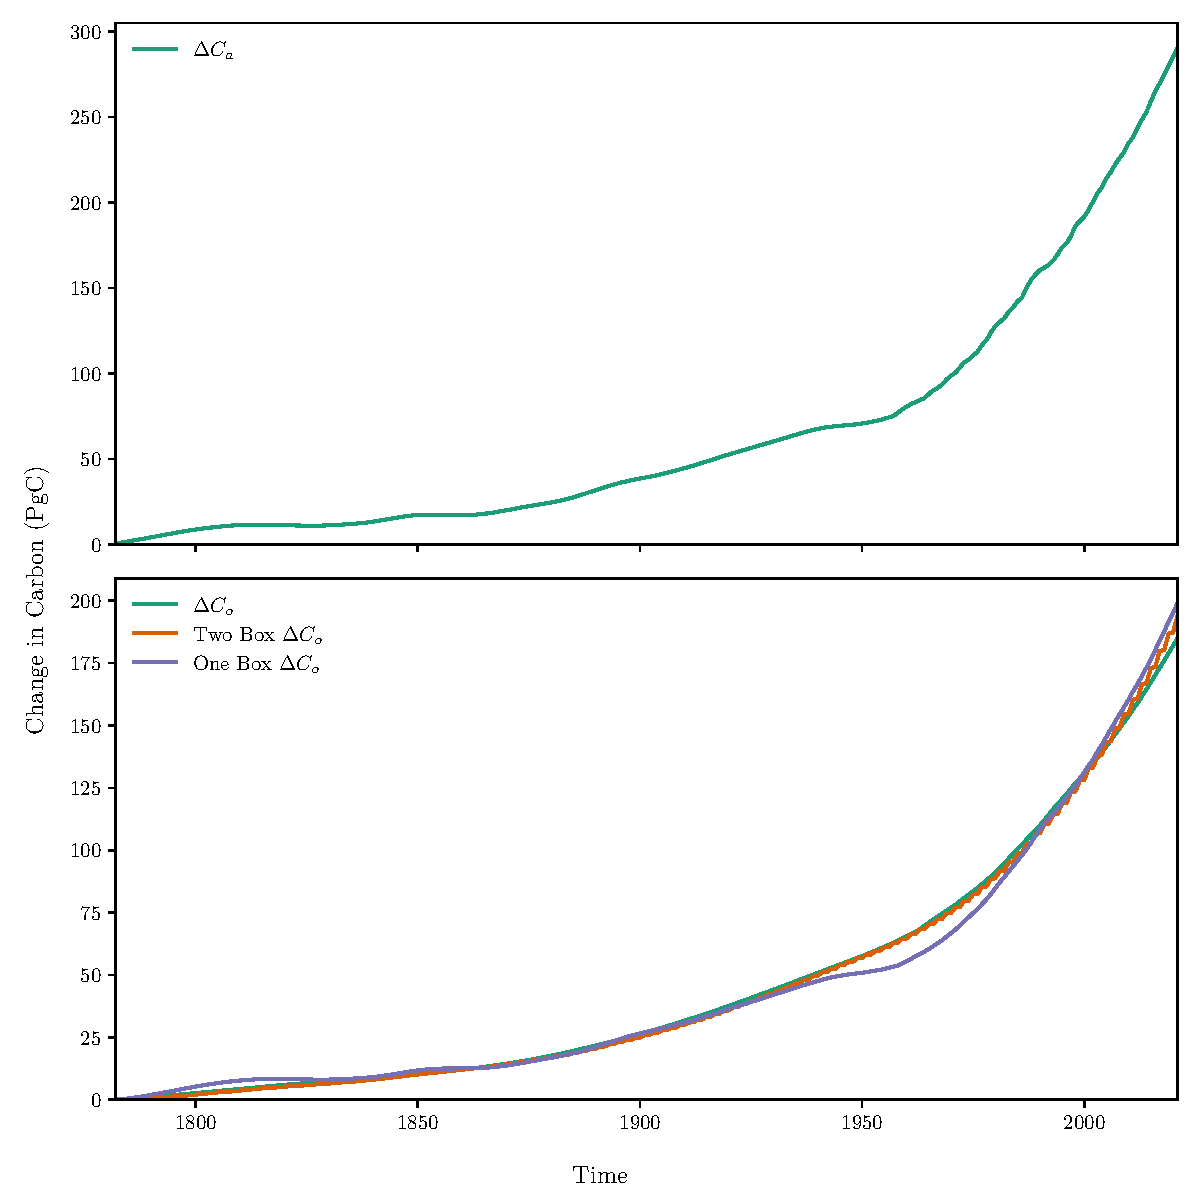
\includegraphics[keepaspectratio,width=\textwidth]{gcb_ocean_atmosphere_boxes}
  \caption{The reconstructed ocean uptake using the one and two box models, with parameters from \cref{tab:one_and_two_box_parameters}}
  \label{fig:fits_from_one_and_two}
\end{figure}


These fits are plotted in \cref{fig:fits_from_one_and_two}. It can be seen that both one and two box models do a reasonable job in captureing the
historical record of ocean carbon uptake. However the two box model does substantially better.

\section{One Box Ocean}
Although the two-box ocean model does better than the one box ocean model in fitting the observed carbon sink, the one box model is simpler
and more easily analysable. Therefore as a warm up, I will analyse the stability of the carbon cycle assuming a one box ocean.

I assume Net Primary Priductivity,$\Pi$, is a function of the atmospheric carbon only. I model heterotrophic respiration as having a $Q_{10}$ temperature dependence:
$R_h = r_0 C_s e^{\alpha T}$ where $r_0$ is the specific respiration, $\alpha = \log \left( Q_{10} \right)/10$ and $C_s$ is the soil carbon. The global temperature anomaly, $T$,
is set assuming a logarithmic dependence on atmospheric \ce{CO2} giving $T = S \log \left(C_a / C_{a0}\right)/\log 2$ where $C_a$ is the atmospheric carbon, $C_{a0}$ is a refernce level of
atmospheric carbon which I take as corresponding to the preindustrial state, which I assume is stable. The parameter $S$ is related to the climate sensitivity, although it is land-weighted.
I set $r_0 = \Pi(C_{a0})/C_{s0}$ where $C_{s0}$ is a reference level of soil carbon, set to the preindustrial level.  

The ocean carbon dynamics are set by the one box model described in \cref{eq:ocean_box_i} and the level of atmospheric carbon is set through conservation of carbon, namely $\mathcal{C} = C_a + C_s + C_o$,
where the total carbon in the atmosphere-land-ocean system to $\mathcal{C}$.

These assumptions give rise to the following set of equations.
\begin{subequations}
  \label{eq:one_box_ocean}
  \begin{align}
    \dv{C_s}{t} &= \Pi(C_a) - r_0 C_s \left(\frac{C_a}{C_{a0}}\right)^{\mu} \\
    \dv{C_o}{t} &= k(C_a - C_{a0}) - \frac{C_o}{\tau} \\
    C_a &= \mathcal{C} - C_s - C_o.
\end{align}
\end{subequations}
The parameter $\mu = \alpha S / \log 2$ will be the control parameter that determines the stability of the system.
Note that there is a fixed point at $C_a = C_{a0}$, $C_o = 0$ and $C_s = C_{s0}$. I am interested in its stability.
\subsection{The Stability of a fixed point}
Here I give a summary of the conditions for an equilibrium to stable. Let
\begin{equation}
  \label{eq:generic_system}
  \dv{\bm{x}}{t} = f(\bm{x})
\end{equation}
with $\bm{x} \in \mathbb{R}^n$ and $f: \mathbb{R}^n \rightarrow \mathbb{R}^n$. Suppose there is a fixed point at $\bm{x}^*$, so $f(\bm{x}^*) = \bm{0}$. Then linearising around this
fixed point gives
\begin{equation}
  \label{eq:generic_system_linearised}
  \dv{\bm{y}}{t} = J\bm{y}
\end{equation}
where $\bm{y} = \bm{x} - \bm{x}^*$ and $J$ is the Jacobian defined by
\begin{equation}
  \label{eq:generic_jacobian}
  J_{ij} = \pdv{f_i}{x_j}.
\end{equation}
This fixed point is stable if no eigenvalues of $J$, denoted $\gamma$, have positive real part.
\subsection{Stability of One Box}
The Jacobian of \cref{eq:one_box_ocean} is given by
\begin{equation}
  \label{eq:jacobian_of_one_box}
    \bm{J} = 
    \begin{pmatrix}
    r_0 \left( \mu \frac{C_{s0}}{C_{a0}} - 1\right) - \Pi'(C_{a0}) & 
    \mu \frac{C_{s0}}{C_{a0}} - \Pi'(C_{a0}) \\
    -k & -k - \frac{1}{\tau}
    \end{pmatrix}
  \end{equation}
where $\Pi'(C_a)$ denotes there derivative of NPP with respect to atmospheric carbon.
  
To finds the eigenvalues of the Jacobian, I must solve the characteristic polynomial $\det(\bm{J} - \gamma \bm{I})$ = 0, where $\gamma$ is an eigenvalue.

This equation is quadratic and therefore has two roots. Solving it leads to a solution of the form:
\begin{equation}
  \label{eq:eigenvalues_of_one_box_jac}
  \gamma_{\pm} = \frac{B \pm \sqrt{\Delta}}{2\tau C_{a0}}
\end{equation}
where
\begin{equation}
  \label{eq:B_in_one_box}
  B = -k \tau  C_{a0}-\Pi'(C_{a0}) \tau  C_{a0}-r_0 \tau  C_{a0}-C_{a0}+\mu  \Pi_0 \tau
\end{equation}
and
\begin{equation}
  \label{eq:discriminant_from_one_box}
  \Delta = \left(k \tau  C_{a0} +\Pi'\tau  C_{a0}+r_0 \tau  C_{a0}+C_{a0}-\mu  \Pi_0 \tau \right)^2-4 \left(k r_0 \tau ^2 C_{a0}^2+\Pi' \tau  C_{a0}^2-\mu  \Pi_0 \tau  C_{a0} +r_0 \tau  C_{a0}^2\right)
\end{equation}
is the discriminant. I have used $\Pi_0 = r_0 C_{s0}$.

The stability of this system is goverened by $\Re \gamma$. This number is controlled by the sign of $\Delta$. If $\Delta > 0$, then $\Re \gamma = \gamma$, but if $\Delta < 0$, then
$\Re \gamma = B / 2\tau C_{a0}$. 

\subsection{Real Eigenvalues}
If $\tau < 1/r_0$ then $\Delta > 0$ for all values of $\mu$. As $1/r_0 \approx 30$ year this situation represents a relatively fast ocean response.
Under this assumption, it turns out that $\gamma_+ > 0$ when
\begin{equation}
  \label{eq:instability_condition_one_box_fast}
  \mu^* = \frac{C_{a0}}{C_{s0}} + \frac{C_{a0}}{\Pi_0} \dv{\Pi}{C_a} + \frac{C_{a0}}{C_{s0}} k\tau.
\end{equation}
It is interesting to compare this to the condition given in \cref{eq:mu_infinity}. If the parameter $\chi_0$ is introduced and set to $\chi_0 = k \tau$.
then \cref{eq:instability_condition_one_box_fast} is identitical to \cref{eq:mu_infinity}. This gives an interpretation to $\chi_0$ as the ratio of the timescale of the ocean carbon flux
to the timescale of its response. Previously, $\chi_0$ was interpreted as a fraction. This can be done only if $\tau < 1/k = \SI{5}{\year}$.
\begin{figure}
  \centering
  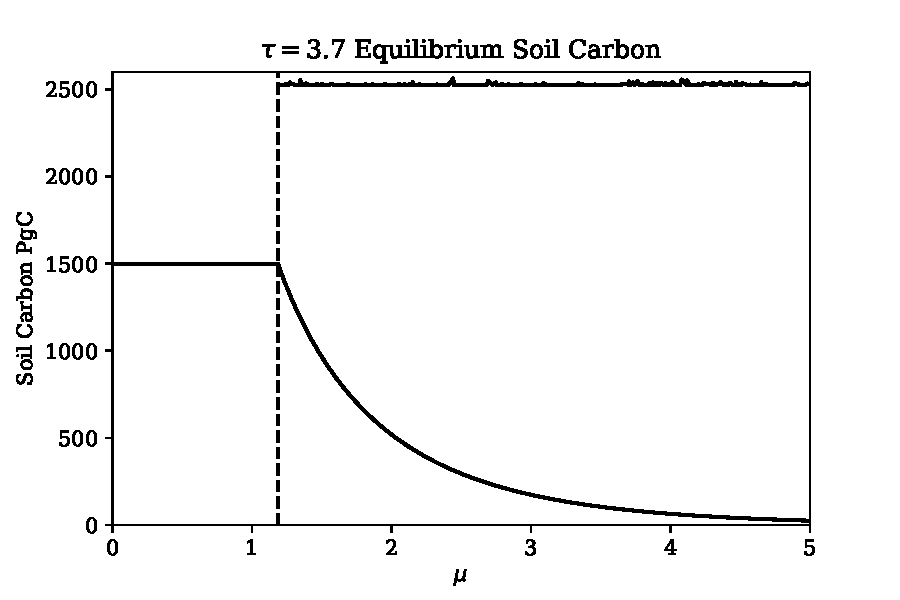
\includegraphics[keepaspectratio,width=\textwidth]{one_box_model_soil_carbon_equilibrium_tau_3.7.pdf}
  \caption{Equilibrium Soil Carbon level as a funtion of $\mu$ for a fast ocean response}
  \label{fig:fast_response_bf_diagram}
\end{figure}

The system \cref{eq:one_box_ocean} is integrated to equilibrium and the equilibria are plotted as a function of $\mu$ in \cref{fig:fast_response_bf_diagram}.
In this case, $\tau = \SI{3.7}{\year}$. The dashed line represents the position
of the analytically calculated bifurcation point. It can been seen that the agreement is good. To the extent that this model is valid, this imposes an upper limit on the possible value of $\mu$ given
the observed stability of the pre-industrial climate.

\subsection{Complex Eigenvalues}
If $\Delta < 0$, which is to say if the ocean response is considered on a long timescale, the stabilty of the system is given by the sign of $B$.
This leads to the condition
\begin{equation}
  \label{eq:instability_condition_one_box_slow}
  \mu^* =\frac{C_{a0}}{C_{s0}} + \frac{C_{a0}}{\Pi_0} \dv{\Pi}{C_a} + \frac{C_{a0}}{C_{s0}} k\tau\left(
     1 + \frac{1}{k\tau}
  \right) \frac{1}{r_0\tau}
\end{equation}
This corresponds to the eigenvalues crossing the imaginary axis and is thus a Hopf bifurcation.

\subsection{Comparison with Data}
For the one box case, it was found that $\tau r_0 \approx 0.1$ which means that the system is in the `real eigenvalues' case. The value of $\chi_0$ becomes
$0.7$.

\missingfigure{One Box Bifurcation Diagram}

\section{Two Box Model}
Suppose I modify \cref{eq:one_box_ocean} to include an extra ocean box. I imagine a fast box and a slow box. In principle, I could repeat the
analysis above, by finding the eigenvalues of a $3 \times 3$ matrix. This is possible in principle but involves solving a cubic polynomial which
is challenging analytically.

Instead, I will use the timescale seperation between the two ocean boxes to make some remarks about the qualitative behaviour of the system.
As the slow box is much slower than the fast box, over short timescales it can be ignored. So if $\mu$ were to be slowly increased through
the condition given in \cref{eq:instability_condition_one_box_fast} there would still be an instability.

However, on longer timescales, the system will still behave like a one box model but now the box will be the slow ocean component. As this is the slow box,
it will have $\Delta < 0$ and so there will be oscillatory behaviour. Hence I expect the bifurcation to occur at a similar place as in the one box fast ocean model,
but to have the character of a Hopf bifurcation.

To be more formal, consider the system
\begin{subequations}
  \begin{align}
    \label{eq:two_box_ocean}
    \dv{C_s}{t} &= \Pi(C_a) - r_0 C_s \left(\frac{C_a}{C_{a0}}\right)^{\mu} \\
    \dv{C_1}{t} &= fk(C_a - C_{a0}) - \frac{C_1}{\tau} \\
    \dv{C_2}{t} &= (1-f)k(C_a-C_{a0}) - \epsilon\frac{C_2}{\tau} \\
    C_a &= \mathcal{C} - C_s - C_1 - C_2
  \end{align}
\end{subequations}
where $f$ is the fraction of carbon taken up by the fast response and $\epsilon$ is the ratio of the timescale of the fast box to the slow box, so $\epsilon \ll 1$. If
$C_2$ can be taken as approximately constant, then there is an instability when $\mu^*_{\mathrm{fast}} = \frac{C_{a0}}{C_{s0}} + \frac{C_{a0}}{\Pi_0} \dv{\Pi}{C_a} + \frac{C_{a0}}{C_{s0}} kf\tau$.

Now working on the slower timescale where $C_1$ is approximately constant the eigenvalues of the Jacobian of $C_s$ and $C_2$ can be evaluated at $\mu = \mu^*_{\mathrm{fast}}$. In this case, the eigenvalues
have the form
\begin{equation}
  \label{eq:slow_eigenvalues}
  \gamma_{\pm} = \frac{f k r_0 \tau ^2+\sqrt{\left(-f k r_0 \tau ^2-f k \tau +k \tau +\epsilon \right)^2-4 \left(-f k r_0 \tau ^2-f k r_0 \tau ^2 \epsilon +k r_0 \tau ^2\right)}+f k \tau -k \tau -\epsilon }
  {2 \tau }.
\end{equation}
For oscaillatory solutions, the arguemnt of the square root must be negative, which requires
\begin{equation}
  \label{eq:epsilon_requirement}
  \epsilon < 2 \sqrt{-f^2 k^2 r_0 \tau ^3+f k^2 r_0 \tau ^3-f k r_0 \tau ^2+k r_0 \tau ^2}-f k r_0 \tau ^2+f k \tau -k \tau.
\end{equation}
For $f = 0.3$, $\tau = 5$ this implies that $\epsilon < 0.06$, which is consistent with the assumption that the second ocean box is slow. This value of $\epsilon$ implies a second box timescale
of about 80 years.
\subsection{Computation of Bifurcation Point}
There is another mode of attack however. The characteristic polynomial of the Jacobian of \cref{eq:two_box_ocean} will be of the form
\begin{equation}
  \label{eq:generic_cubic}
  \gamma^3 + a_1 \gamma^2 + a_2 \gamma + a_3 = 0.
\end{equation}
At the Hopf bifurcation, $\gamma$ is purely imaginary, so set $\gamma = i\lambda$. Then \cref{eq:generic_cubic} becomes
\begin{equation}
  \label{eq:cubic_with_imaginary_root}
  -i\lambda^3 - a_1 \lambda^2 + i a_2 \lambda + a_3 = 0. 
\end{equation}
Demanding that both real and imaginary parts of \cref{eq:cubic_with_imaginary_root} are zero, leads to $\lambda = \pm \sqrt{a_3/a_1}$ and $\lambda = \pm \sqrt{a_2}$. That these two expressions
are equal leads to the condition that $a_3 = a_1a_2$, which can then be solved for $\mu$. Doing this gives
\begin{equation}
  \label{eq:mu_two_box}
  \begin{split}
  \mu^* = &\frac{C_{a0}}{2 \Pi_0 \tau  (1+\epsilon)}
  \Biggl(
  -f k \tau  (1-\epsilon)+r_0 \tau  (2 + k \tau +2 \epsilon)+k \tau  (2+\epsilon)+(1+\epsilon) (1+2 \Pi' \tau +\epsilon)\\
  &\pm\sqrt{
    \begin{split}
    f^2 k^2 \tau ^2 (1-\epsilon)^2-&2 f k \tau  (1-\epsilon) \left(r_0 \tau  (k \tau +2 \epsilon +2)-k \tau  \epsilon -(1+\epsilon)^2\right)\\+
    \left(1+k r_0 \tau ^2-k \tau  \epsilon -\epsilon ^2\right)^2
  \end{split}}
  \Biggr)
  \end{split}
\end{equation}
or
\begin{equation}
  \label{eq:mu_two_box_zero_eps}
  \begin{split}
  \mu^* \sim &\frac{C_{a0}}{\Pi_0}\Biggl(
    \frac{1}{2\tau} + k(1 - \frac{1}{2}f + \frac{1}{2}r_0 \tau) + r_0 + \Pi'\\
    &\pm\frac{1}{2}\sqrt{\frac{1}{\tau^2} + \frac{2kf}{\tau} + k(kf^2 + 2 (1 - 2f)r_0  - 2 k r_0\tau f  + k r_0^2 \tau^2)}\,\Biggr)
\end{split}
\end{equation}
as $\epsilon \rightarrow 0$.
There are 2 values of $\mu$ that satisfy the consistency condition --- there are two Hopfs? (Sub/supercritical?)
In the case where $\epsilon = 0$ and $f = 1$, this reduces to the one box model case. In this case \cref{eq:mu_two_box} becomes
\begin{equation}
  \label{eq:mu_zero_one}
  \mu^*_{\pm} = \frac{C_{a0} \left(\pm\left(-k r_0 \tau ^2+k \tau +1\right)+r_0 \tau  (k \tau +2)+k \tau +2 \Pi' \tau +1\right)}{2 \Pi_0 \tau}
\end{equation}
or
\begin{align}
  \label{eq:mu_zero_one_cases}
  \mu_+^* &= \frac{C_{a0}}{C_{s0}} + \frac{C_{a0}}{\Pi_0}\dv{\Pi}{C_a} + \frac{C_{a0}}{C_{s0}} \left(\frac{k}{r_0} + \frac{\tau^{-1}}{r_0}\right) \\
  \mu_-^* &= \frac{C_{a0}}{C_{s0}} + \frac{C_{a0}}{\Pi_0}\dv{\Pi}{C_a} + \frac{C_{a0}}{C_{s0}}k\tau 
\end{align}
which correspond to the conditions (\cref{eq:instability_condition_one_box_fast,eq:instability_condition_one_box_slow}) derived for the one box case.

\missingfigure{Eigenvalues of Jacobian Demonstrating Spurious Root}
\missingfigure{Bifurcation Diagram with fitted parameters}

\section{IMOGEN}
\subsection{IMOGEN description}
\subsection{Bifurcations in IMOGEN}
\missingfigure{Bifurcation Diagram for IMOGEN}
\subsection{Variability in IMOGEN}
\begin{subequations}
  \label{eq:climate_system}
  \begin{align}
    c_1 \dv{T_1}{t} &= \frac{Q_{2\times}}{\log 2} \log \frac{C_a}{C_{a0}} - \frac{Q_{2\times}}{ECS}T_1 -\gamma (T_1 - T_2) + \sigma_Q \xi(t)\\
    c_2 \dv{T_2}{t} &= -\gamma(T_1 - T_2) \\
    \dv{C_s}{t}     &= \Pi(C_a) - C_s r_0 e^{\alpha T_1} \\
    \dv{C_o}{t}     &= \mathrm{IMOGEN} \\
    C_a &= \mathcal{C} - C_s - C_o
  \end{align}
\end{subequations}